\documentclass[11pt]{article}

\usepackage[utf8]{inputenc}
\usepackage[T1]{fontenc}
\usepackage[margin=1in]{geometry}
\usepackage{lmodern}
\usepackage{microtype}
\usepackage{amsmath,amssymb}
\usepackage{booktabs}
\usepackage{array}
\usepackage{enumitem}
\usepackage{xcolor}
\usepackage{hyperref}
\usepackage{tikz}
\usetikzlibrary{arrows.meta, positioning, shapes.geometric, fit}
\usepackage{tcolorbox}
\usepackage{caption}
\usepackage{float}

\hypersetup{
  colorlinks=true,
  linkcolor=blue!55!black,
  citecolor=blue!55!black,
  urlcolor=blue!65!black,
  pdftitle={A Source-Gated Representation of the 2026 Offshore Sarangani Sequence},
  pdfauthor={Chief, working research draft}
}

\tcbset{
  claimbox/.style={
    colback=gray!6,
    colframe=black!70,
    boxrule=0.7pt,
    arc=2pt,
    left=8pt,
    right=8pt,
    top=8pt,
    bottom=8pt,
    before skip=10pt,
    after skip=10pt
  }
}

\tikzset{
  gate/.style={rectangle, rounded corners, draw=black!70, fill=gray!8, minimum width=3.0cm, minimum height=0.9cm, align=center, font=\small},
  waitgate/.style={rectangle, rounded corners, draw=orange!70!black, fill=orange!10, minimum width=3.0cm, minimum height=0.9cm, align=center, font=\small},
  nogo/.style={rectangle, rounded corners, draw=red!60!black, fill=red!7, minimum width=3.0cm, minimum height=0.9cm, align=center, font=\small},
  arrow/.style={-{Stealth[length=5pt]}, thick, draw=black!75}
}

\title{\textbf{A Source-Gated Representation of the 2026 Offshore Sarangani Sequence}\\[4pt]
\large Aftershock Geometry, Marine-Gravity Residuals, Coastal-Uplift Evidence, and Claim Boundaries}

\author{Chief Research Draft\\
\small Internal source-grounded manuscript, v0.1}

\date{June 2026}

\begin{document}
\maketitle

\begin{abstract}
The 08 June 2026 offshore Sarangani earthquake sequence motivates a difficult research problem: a visible aftershock corridor, regional coastal-uplift reports, focal-mechanism context, slab geometry, and marine-geophysical residuals appear mutually relevant, yet the strongest local source layers remain unavailable or incomplete. This draft proposes a source-gated representation of the problem. Rather than treating the sequence as proof of a named offshore structure, prediction capability, or inherited tectonic-memory mechanism, the paper organizes current evidence into gates: public PHIVOLCS bulletin geometry, SWIFT-CMT mechanism context, Slab2 and active-fault controls, ETOPO/EMAG2 screening, UCSD/SIO marine-gravity residuals, NAMRIA hydrographic acquisition, Kitayo/Jose Abad Santos coastal-uplift evidence, and PHIVOLCS aftershock-catalog completeness. The current synthesis is conservative: the marine-gravity residual survives exact mapped-active-fault and normalized Slab2 absolute-depth controls, but the distance effect becomes tight and the corridor-parallel orientation signal is the cleaner residual. Regional coseismic coastal uplift is source-backed through PHIVOLCS/MGB/DENR/PENRO-linked reporting, but exact Kitayo geometry, tide-corrected displacement, official bathymetry, and a named causative offshore structure remain unresolved. The contribution of this draft is therefore not a mechanism verdict. It is a disciplined representation of what can be claimed, what remains inferential, and what source-grade evidence would be required to raise the claim ceiling.
\end{abstract}

\begin{tcolorbox}[claimbox]
\textbf{Standing verdict.} The current evidence state is \emph{underdetermined}: strong enough to investigate, not strong enough to claim. The strongest allowed claim is that a source-backed regional uplift observation and a matched-null-surviving marine-gravity residual justify further source acquisition and stricter modeling. They do not establish causation, prediction capability, inherited-memory proof, or a named offshore controlling structure. Machine-verifiable boundary: the draft does not establish causation, prediction capability, inherited-memory proof, or a named offshore controlling structure.
\end{tcolorbox}

\section{Introduction}

The 08 June 2026 offshore Sarangani earthquake produced a dense public record of aftershocks, focal-mechanism products for a subset of larger events, regional coastal-uplift reporting, and renewed attention to the Cotabato Trench--Celebes Sea margin. These observations invite a natural but dangerous question: does the spatial organization of the sequence reveal a local offshore structure or deeper tectonic memory? The available evidence does not yet support that conclusion. It supports a more careful claim: the sequence is structured enough to investigate, while the decisive local source layers remain missing.

This paper draft encodes the research as a sequence of evidence gates. A gate is not a rhetorical section; it is a claim-control device. It states what a source class supports, what it weakens, and what it cannot carry. The method is motivated by a recurring failure mode in earthquake interpretation: a valid local observation can become an invalid causal claim if moved across evidentiary levels without new source support.

The present manuscript has three goals:
\begin{enumerate}[leftmargin=2em]
  \item summarize the current source-grounded TMCH evidence chain;
  \item preserve the boundary between observation, inference, hypothesis, and blocked claims;
  \item define the specific source acquisitions needed before mechanism claims can be strengthened.
\end{enumerate}

The paper is intentionally written as a source-gated research draft, not a final geologic interpretation.

\section{Source Basis and Claim Discipline}

The draft is based on internal TMCH artifacts and bounded public/official source captures. The source basis includes PHIVOLCS public earthquake bulletins, PHIVOLCS SWIFT-CMT source-parameter pages, NOAA/NCEI ETOPO relief, NOAA/NCEI EMAG2 magnetic-anomaly screening, UCSD/SIO marine gravity, USGS Slab2 regional slab geometry, PHIVOLCS/GeoRiskPH active-fault geometry, NAMRIA/OMSIS chart and ENC acquisition channels, source-backed media reports quoting or describing PHIVOLCS/MGB/DENR/PENRO coastal-uplift observations, and the Imamura--Omori quasi-cycle doctrine derived from Geller's historical analysis of earthquake-forecasting claims \cite{phivolcs-latest,phivolcs-swift,namria-products,etopo,emag2,sandwell,slab2,geller2023,tmch-v05,kitayo-ladder,namria-gate,phivolcs-catalog-gate}.

\subsection{Claim levels}

We distinguish four levels:
\begin{description}[leftmargin=2.6cm,style=nextline]
  \item[Observation] Public or source-backed record: bulletin rows, reported field observations, source products, artifact outputs.
  \item[Inference] Reasoned interpretation from current evidence: for example, a residual that survives matched controls may indicate a missing local source layer.
  \item[Hypothesis] Plausible but unverified mechanism: for example, upper-plate splay faulting or basin/basement contrast as an explanation for an offshore residual.
  \item[Blocked claim] A conclusion not currently supported: named causative offshore fault, exact Kitayo displacement, inherited-memory proof, or prediction capability.
\end{description}

\begin{table}[H]
\centering
\caption{Claim boundary ledger. The core function of the research frame is to prevent evidence-class mixing.}
\label{tab:claim-ledger}
\begin{tabular}{p{0.26\linewidth}p{0.31\linewidth}p{0.31\linewidth}}
\toprule
\textbf{Evidence class} & \textbf{Allowed wording} & \textbf{Not allowed} \\
\midrule
PHIVOLCS public bulletin table & Working row-level bulletin extraction with time, location, depth, magnitude & Official associated-aftershock sequence completeness \\
Regional uplift reports & PHIVOLCS/MGB/PENRO-linked reporting supports regional coseismic uplift & Exact Kitayo uplift at a measured field coordinate \\
Marine-gravity matched null & Residual survives exact active-fault and normalized Slab2 controls & Marine gravity caused the rupture \\
NAMRIA product identifiers & Official acquisition path and chart/ENC targets identified & NAMRIA bathymetry confirms offshore structure \\
TSRA/quasi-cycle doctrine & Weak observation scaffold and preparedness prior & Earthquake prediction capability \\
Historical chart workspace & Visual/provenance context after failed extraction QA & Accepted bathymetry or structural vector evidence \\
\bottomrule
\end{tabular}
\end{table}

\section{Problem Representation}

The research problem is not simply whether a north--south aftershock corridor is visible. The harder question is whether that corridor remains meaningful after accounting for ordinary active-margin structure, mapped active faults, modeled slab geometry, detection/completeness limitations, and missing local offshore data.

The working representation is therefore:
\begin{quote}
\emph{an active-margin residual-structure problem under strict source gates.}
\end{quote}

This representation makes several operations cheap: null design, evidence ranking, source acquisition, and claim-ceiling enforcement. It makes one operation deliberately expensive: mechanism closure. Mechanism closure should remain expensive until the missing source layers arrive.

\subsection{What this representation avoids}

The representation rejects five shortcuts:
\begin{enumerate}[leftmargin=2em]
  \item treating aftershock alignment as a rupture-vector or subduction-vector by default;
  \item transferring regional uplift measurements directly to Kitayo;
  \item treating NAMRIA identifiers as acquired bathymetry;
  \item treating failed PNG-derived chart extraction as weak evidence;
  \item treating temporal observation windows as forecasts.
\end{enumerate}

\section{Current Evidence Gates}

\subsection{Public PHIVOLCS bulletin geometry}

PHIVOLCS Latest Earthquake Information provides official public bulletin rows including date/time, latitude, longitude, depth, magnitude, and location text \cite{phivolcs-latest}. The internal PHIVOLCS catalog acquisition gate records that the table includes the main event row:
\begin{quote}
08 June 2026, 07:37 AM; latitude $5.57^\circ$N; longitude $124.98^\circ$E; depth 33 km; magnitude 7.8; approximately 32 km S $04^\circ$ W of Maasim, Sarangani \cite{phivolcs-catalog-gate}.
\end{quote}

This public table is useful for a working geometry surface. It is not an official associated-aftershock sequence export. The missing field is not merely a coordinate; it is the association and completeness metadata that would separate true sequence rows from unrelated Philippine events in the same date table.

\subsection{SWIFT-CMT mechanism context}

PHIVOLCS SWIFT-CMT source-parameter products provide a subset of waveform-inversion source locations and mechanisms, with fields such as UTC date, longitude, latitude, depth, moment magnitude, location, and analysis type \cite{phivolcs-swift}. Internal TMCH synthesis treats these as mechanism evidence for larger or solved events, not as a full aftershock catalog. The mechanism subset strengthens ordinary active-margin interpretations but does not prove a named local source.

\subsection{Slab2 and mapped active-fault controls}

USGS Slab2 provides modeled regional slab geometry, and PHIVOLCS/GeoRiskPH active-fault geometry provides mapped active-fault context. In the TMCH workflow, a key methodological progression was replacing coarse active-fault midpoint proximity with exact PHIVOLCS active-fault polyline distance, then rerunning the marine-gravity matched null with Slab2 depth normalized as absolute depth \cite{tmch-v05}. This corrected a sign-convention concern and produced a tighter but still surviving residual.

\subsection{Marine-gravity residual}

The strongest current residual class is the UCSD/SIO marine-gravity gradient screen. Under the normalized-Slab2 exact-active-fault matched null, the observed median high-gradient gravity distance was 6.6846 km versus a matched-null median of 7.3900 km. The distance component therefore survives but becomes much tighter than the earlier exact-fault version suggested. The corridor-parallel axis fraction remains cleaner: observed 0.4116 versus matched-null median 0.3370 \cite{tmch-v05}.

The disciplined interpretation is not that gravity caused rupture. It is that the residual may be screening a local offshore structural organization not captured by currently available mapped active-fault and slab geometry layers.

\subsection{Coastal-uplift evidence}

The Kitayo/Jose Abad Santos uplift lane is now source-gated. PHIVOLCS/MGB/DENR/PENRO-linked reporting supports regional coseismic coastal uplift affecting southern Glan and Jose Abad Santos, and preliminary reports include approximately 2 m uplift and about 200 m shoreline retreat in at least one reported affected area such as Pangyan/Glan \cite{kitayo-ladder}. This is not the same as exact Kitayo displacement. The Kitayo QGIS point remains an approximate barangay-level observation anchor, not a field GPS point or official exposed-shoreline coordinate.

\subsection{NAMRIA hydrographic acquisition}

NAMRIA products and OMSIS/ENC availability channels identify the correct official hydrographic acquisition path. Current WGS-84 chart targets include chart 1524, Sarangani Bay to Calian Point, and chart 1525, Tuna Point to Sarangani Bay; ENC PH2CMN40, Central Mindanao, is the best broad regional ENC target identified so far \cite{namria-gate,namria-products}. Legacy chart 4607 is useful for provenance/context only, and withdrawn chart 4608 should not be used as current evidence.

The key boundary is simple: NAMRIA chart/ENC availability is not acquired bathymetry. The next step is request/acquisition, metadata audit, and then QGIS import.

\section{Evidence-Gated Research Architecture}

Figure~\ref{fig:gates} summarizes the current research architecture. The structure intentionally separates working evidence from waiting gates and blocked claims.

\begin{figure}[H]
\centering
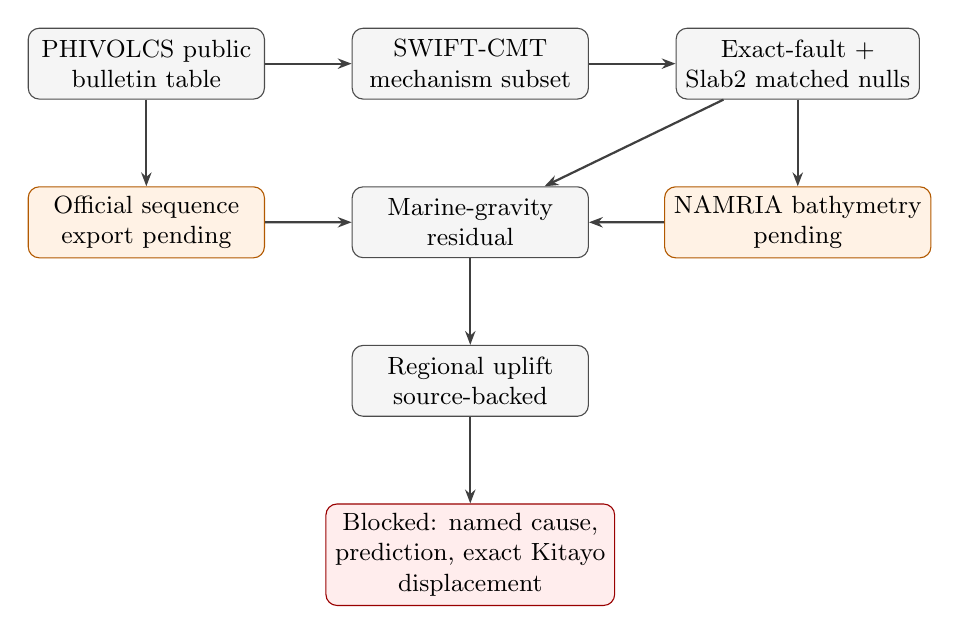
\begin{tikzpicture}[node distance=1.1cm and 1.1cm]
  \node[gate] (bulletin) {PHIVOLCS public\\bulletin table};
  \node[gate, right=of bulletin] (mechanism) {SWIFT-CMT\\mechanism subset};
  \node[gate, right=of mechanism] (nulls) {Exact-fault +\\Slab2 matched nulls};
  \node[gate, below=of mechanism] (residual) {Marine-gravity\\residual};
  \node[waitgate, below=of bulletin] (catalog) {Official sequence\\export pending};
  \node[waitgate, below=of nulls] (namria) {NAMRIA bathymetry\\pending};
  \node[gate, below=of residual] (uplift) {Regional uplift\\source-backed};
  \node[nogo, below=of uplift] (blocked) {Blocked: named cause,\\prediction, exact Kitayo\\displacement};

  \draw[arrow] (bulletin) -- (mechanism);
  \draw[arrow] (mechanism) -- (nulls);
  \draw[arrow] (nulls) -- (residual);
  \draw[arrow] (bulletin) -- (catalog);
  \draw[arrow] (nulls) -- (namria);
  \draw[arrow] (catalog) -- (residual);
  \draw[arrow] (namria) -- (residual);
  \draw[arrow] (residual) -- (uplift);
  \draw[arrow] (uplift) -- (blocked);
\end{tikzpicture}
\caption{Source-gated representation of the current TMCH research state. Solid evidence gates support working synthesis; orange gates indicate pending official acquisitions; the red gate marks claims that remain blocked without new source-grade evidence.}
\label{fig:gates}
\end{figure}

\section{Matched-Null Residual Interpretation}

The marine-gravity result is most useful when framed as a residual under controls, not as a causal mechanism. The sequence of nulls changed the interpretation. Early random or weakly matched comparisons suggested a stronger distance relationship between aftershocks and gravity gradients. After exact active-fault polyline distance and normalized Slab2 absolute-depth matching, the distance component tightened substantially, while the corridor-parallel orientation component remained comparatively cleaner \cite{tmch-v05}.

This produces a narrow inference:
\begin{quote}
The residual is compatible with a local structural organization of the active margin that is not yet represented in the available public structural layers.
\end{quote}

It does not establish which structure is responsible. Candidate classes include upper-plate splays, frontal-wedge or trench-segmentation structures, forearc/basin-basement density contrasts, Cotabato Fault/SCDL-related shear partitioning, or other local offshore lineaments. These remain candidate classes, not selected mechanisms.

\section{Coastal Uplift and the Kitayo Boundary}

The uplift thread adds important context, but it also raises the risk of overclaiming. The evidence ladder distinguishes regional source-backed uplift from exact Kitayo geometry. Regional coastal uplift after the event is now supported by PHIVOLCS/MGB/DENR/PENRO-linked reporting, but the following remain unresolved: exact Kitayo location, tide-corrected displacement, vertical datum, field GPS or polygon, before/after satellite shoreline trace, and a source-backed local offshore causative structure \cite{kitayo-ladder}.

The disciplined wording is:
\begin{quote}
Kitayo is an approximate observation anchor within a broader source-backed regional uplift context.
\end{quote}

The undisciplined wording is:
\begin{quote}
Kitayo rose by the reported regional measurement, or a named offshore splay caused the local uplift.
\end{quote}

The latter should not be used in the current evidence state.

\section{Acquisition Gates}

Two acquisition gates now define the research ceiling.

\subsection{NAMRIA hydrographic gate}

The NAMRIA gate asks for official chart/ENC/bathymetric products. Its purpose is to replace failed historical PNG extraction with official hydrographic evidence. The current target set includes charts 1524 and 1525, ENC PH2CMN40, and possible hydrographic smooth sheets or nautical feature digital data for the Sarangani Bay--Jose Abad Santos--Kitayo area \cite{namria-gate}.

\subsection{PHIVOLCS aftershock sequence gate}

The PHIVOLCS aftershock-catalog gate asks for source-grade row-level sequence data: event ID or sequence ID, origin time, latitude, longitude, depth, magnitude, magnitude type, location, association with the 08 June 2026 sequence, review status, solution quality, and completeness/detection-threshold metadata \cite{phivolcs-catalog-gate}. This is foundational for any later corridor-axis, depth, timing, or completeness-controlled spatial analysis.

\section{Temporal Doctrine: Quasi-Cycles as Observation Scaffolds}

The TSRA/TMCH temporal doctrine borrows from the Imamura--Omori historical debate as analyzed by Geller: apparent quasi-cyclicity may support preparedness and observation, but it must not be converted into deterministic forecasting authority \cite{geller2023,imamura-omori}. The working doctrine is:
\begin{quote}
quasi-cycles = observation scaffolds, not prophecy.
\end{quote}

This matters because the same discipline applies spatially. A corridor, residual, or uplift observation may guide investigation; it does not, by itself, prove source mechanics.

\section{Discussion}

The current TMCH synthesis is strongest as a method of disciplined attention. It says where to look next and which claims are too expensive to make now. The ordinary active-margin explanation remains the default: Cotabato-margin segmentation, upper-plate splay faulting, forearc basin or basement-contrast structure, and subduction-related mechanics are all more conservative than exotic or prediction-like interpretations.

At the same time, the residual should not be discarded. Marine gravity remains the strongest residual class because it survives several controls and because its orientation structure remains elevated under the corrected null. The right interpretation is neither dismissal nor inflation. It is acquisition pressure: the residual is a reason to acquire NAMRIA-scale bathymetry, offshore structural vectors, sequence association metadata, and completeness controls.

\section{Limitations and Open Questions}

\begin{enumerate}[leftmargin=2em]
  \item The PHIVOLCS event catalog currently available to the research flow is a public-page extraction or bounded public fetch, not an official associated-aftershock sequence export.
  \item Detection and completeness controls are missing.
  \item Several SWIFT-CMT values remain image-derived or OCR-derived and require manual audit.
  \item NAMRIA chart/ENC identifiers are known, but official bathymetry has not been acquired.
  \item Historical chart rasters failed automated contour and sounding extraction QA and remain visual/provenance context only.
  \item Exact Kitayo coastal-uplift geometry, tide correction, and vertical datum remain unresolved.
  \item No named offshore controlling structure is established.
  \item No prediction capability is claimed.
\end{enumerate}

\section{Evaluation Plan}

The next version of this manuscript should be revised only after at least one source gate changes state. The evaluation plan is:
\begin{enumerate}[leftmargin=2em]
  \item obtain or receive PHIVOLCS guidance on associated aftershock sequence data;
  \item obtain NAMRIA chart/ENC/bathymetry/smooth-sheet products or formal availability guidance;
  \item audit SWIFT-CMT source-parameter rows against original images/pages;
  \item import official hydrographic data into QGIS with datum/projection/vertical-datum metadata;
  \item rerun spatial models with exact active-fault distance, normalized slab covariates, land/ocean class, gravity-gradient fields, local offshore vectors, and sequence completeness controls;
  \item update the mechanism-discrimination matrix only after the geometry and completeness gates improve.
\end{enumerate}

\section{Conclusion}

The 2026 offshore Sarangani sequence is strong enough to justify structured investigation. The current evidence supports a source-gated residual frame: aftershock geometry, focal mechanisms, slab geometry, active-fault controls, marine gravity, and regional uplift evidence cohere enough to motivate further acquisition, but not enough to close mechanism. The most important result is therefore epistemic rather than causal: the research now has a disciplined map of what is known, what is inferred, what is hypothesized, and what remains blocked.

The next scientific move is not a stronger story. It is stronger source geometry.

\begin{thebibliography}{99}

\bibitem{phivolcs-latest}
DOST-PHIVOLCS. \emph{PHIVOLCS Latest Earthquake Information}. Public earthquake bulletin table, accessed and summarized in TMCH source artifacts, 2026. URL: \url{https://earthquake.phivolcs.dost.gov.ph/}.

\bibitem{phivolcs-swift}
DOST-PHIVOLCS. \emph{SWIFT-CMT Source Parameters}. Source locations and mechanisms obtained from waveform inversions, accessed and summarized in TMCH artifacts, 2026. URL: \url{http://swift1.phivolcs.dost.gov.ph/~pvjica/events/home_sparameters.html}.

\bibitem{namria-products}
NAMRIA. \emph{Nautical chart, ENC, OMSIS, and hydrographic product pages}. Accessed and summarized in TMCH NAMRIA acquisition gate, 2026. URL: \url{https://www.namria.gov.ph/}.

\bibitem{etopo}
NOAA National Centers for Environmental Information. \emph{ETOPO 2022 Global Relief Model}. Used as regional bathymetry/relief context in TMCH source artifacts.

\bibitem{emag2}
NOAA National Centers for Environmental Information. \emph{EMAG2v3 Earth Magnetic Anomaly Grid}. Used as regional magnetic-anomaly screening context in TMCH source artifacts.

\bibitem{sandwell}
Gevorgian, J., Sandwell, D., Yu, Y., Kim, S.-S., and Wessel, P. Marine gravity and related catalog products used in TMCH residual screening; SIO/UCSD Sandwell gravity-grid context summarized in internal TMCH artifacts.

\bibitem{slab2}
Hayes, G. P. and collaborators. \emph{Slab2: A comprehensive subduction zone geometry model}. USGS slab geometry context used in TMCH matched-null controls.

\bibitem{geller2023}
Geller, R. J. \emph{The Imamura vs. Omori Earthquake Forecasting Debate}. The Asia-Pacific Journal / Japan Focus, 2023. Cambridge Core PDF captured in TMCH/TSRA source context.

\bibitem{tmch-v05}
Chief Research Artifacts. \emph{TMCH Gate Synthesis Memo v0.5}. Internal source-grounded synthesis updated after normalized-Slab2 exact-active-fault marine-gravity null, 2026.

\bibitem{kitayo-ladder}
Chief Research Artifacts. \emph{TMCH Kitayo Uplift Evidence Ladder v0.1}. Internal claim-control synthesis for Kitayo/Jose Abad Santos coastal-uplift evidence, 2026.

\bibitem{namria-gate}
Chief Research Artifacts. \emph{TMCH NAMRIA ENC / Chart Acquisition Gate v0.1}. Internal official hydrographic acquisition-path gate, 2026.

\bibitem{phivolcs-catalog-gate}
Chief Research Artifacts. \emph{TMCH PHIVOLCS Aftershock Catalog Acquisition Gate v0.1}. Internal official sequence-data acquisition gate, 2026.

\bibitem{imamura-omori}
Chief Research Artifacts. \emph{Imamura--Omori Quasi-Cycle Synthesis Memo v0.1}. Internal doctrine note: quasi-cycles as observation scaffolds, not prophecy, 2026.

\end{thebibliography}

\end{document}
